\documentclass[12pt,a4paper]{article}
\usepackage{tabularx}
\usepackage{booktabs}
\usepackage{longtable}
\usepackage{ltxtable}
\usepackage[latin1]{inputenc}
\usepackage{amssymb}
\usepackage[]{graphicx,rotating}
\usepackage[T1]{fontenc}
\usepackage{parskip}
\usepackage{listings}
\usepackage{natbib}
\usepackage[official]{eurosym}
\usepackage{mathrsfs}
\usepackage{amsmath}
\usepackage{verbatim}
\usepackage{epstopdf} % to include eps files


\usepackage[usenames,dvipsnames]{color}     %for R colors and formatting
\usepackage{tikz,pgfplots,pgf}% for drawing neural net
\usepackage{neuralnetwork}
\usetikzlibrary{matrix,shapes,arrows,positioning}

\usepackage[left=3cm, right=2.5cm, top=2.5cm]{geometry}

\pagestyle{empty}
\parindent 0.0cm
\renewcommand{\baselinestretch}{1}
\newcommand{\bs}{\boldsymbol}
\renewcommand{\familydefault}{cmr} % alternative: cmss
\pdfminorversion=7
\bibliographystyle{agsm}
% for formatting packages, R, and Code
\newcommand{\pkg}[1]{{\normalfont\fontseries{b}\selectfont #1}}
\let\proglang=\textsf
\let\code=\texttt

\lstset{ %for R colors and formatting
  language=R,                     % the language of the code
  basicstyle=\scriptsize\ttfamily, % the size of the fonts that are used for the code
  numbers=left,                   % where to put the line-numbers
  numberstyle=\scriptsize\color{Blue},  % the style that is used for the line-numbers
  stepnumber=1,                   % the step between two line-numbers. If it is 1, each line
                                  % will be numbered
  numbersep=5pt,                  % how far the line-numbers are from the code
  backgroundcolor=\color{white},  % choose the background color. You must add \usepackage{color}
  showspaces=false,               % show spaces adding particular underscores
  showstringspaces=false,         % underline spaces within strings
  showtabs=false,                 % show tabs within strings adding particular underscores
  frame=single,                   % adds a frame around the code
  rulecolor=\color{black},        % if not set, the frame-color may be changed on line-breaks within not-black text (e.g. commens (green here))
  tabsize=2,                      % sets default tabsize to 2 spaces
  captionpos=b,                   % sets the caption-position to bottom
  breaklines=true,                % sets automatic line breaking
  breakatwhitespace=false,        % sets if automatic breaks should only happen at whitespace
  keywordstyle=\color{RoyalBlue},      % keyword style
  commentstyle=\color{YellowGreen},   % comment style
  stringstyle=\color{ForestGreen}      % string literal style
} 

\begin{document}

\begin{center}
% \vspace*{1cm}
 
\includegraphics[width=0.35\textwidth]{GU-Logo-blau-CMYK.eps} \vspace{2cm}
  
  {\Large{\bf Predicting Cross-Sell with Artificial Neural Networks}} \newline
  {\Large{An Empirical Study of ING's Customer Data}} \vspace{0.5cm}

  Seminar Thesis \\\vspace{2cm}
  submitted to \\\vspace{0.5cm}
  \textbf{Hon.-Prof. Dr. Martin Schmidberger} \\
  \textbf{Gabriela Alves Werb} \\\vspace{0.5cm}
  Goethe University Frankfurt am Main \\
  School of Business and Economics \\
  Chair for E-Commerce \vspace{2cm}
  
  by \\\vspace{0.5cm}
  \textbf{Lukas J\"urgensmeier} \\
  (Mat.-Nr.: 6904281) \\
  
  \medskip
  \medskip
  in partial fulfillment of the requirements \\
  for the degree of \\\vspace{0.5cm}
  \textbf{Master of Science in Business Administration} \\\vspace{0.5cm}
  July 31, 2019
  
\end{center}


\pagebreak
\pagestyle{plain}
\pagenumbering{Roman}
\tableofcontents
\pagebreak
\listoffigures
\listoftables
\newpage
\setcounter{page}{2}
\pagenumbering{arabic}
\setlength{\baselineskip}{1.5\baselineskip}
\pagestyle{plain}


\section{Introduction}
\citep{hastieElementsStatisticalLearning2017}
Include research question here \\
\pkg{dplyr}
\proglang{R}
\code{a <- mutate(data, abc)}
Identify  addtitional  sales  potential in the client base to increase customer value and loyalty. \newline
Question: Will a customer buy an additional product? (yes/no) \newline
Goal: identify characteristics of typical customers who open a checking account and predict which customers
are likely open a checking account in the future
\section{Theoretical Background on Cross-sell}

\section{Methodology}
This section provides an overview over the implemented methodology by first outlining the feature engineering process that transforms the original data set
as required by neural networks.
The second part then describes the artificial neural network and its initial architecture, while the third part describes the hyperparameter tuning process
that leads to the \textit{best} model\footnote{This model is definitely not the best model \textit{existing}, but the best model \textit{found} through the trial-and-error tuning process.}.
Lastly, this section addresses a common criticism of machine learning technologies in general and neural networks in particular---the 
uninterpretable black box---by introducing the Local Interpretable Model-agnostic Explanation (LIME) as a method to 
"look under the hood" of a neural network and determine which features contributed by how much to a prediction.

\subsection{Feature Engineering and Data Set Preparation}
In order to feed seamlessly into a neural network, extensive feature engineering and data preparation is required \citep{hastieElementsStatisticalLearning2017}.
Before training the model, I replace missing values in \code{pref\_device} and \code{occupation} by \code{None\_or\_missing}, transform all \code{char} variables to a \code{factor} type, and remove the misleading feature \code{ID}.
However, there are still numerous features including missing values. Since they are not missing at random, they need to be dealt with in order to not
bias the prediction.
Deleting all observations with missing values would do exactly that.
Hence, I impute missing values with a Random Forest from the \pkg{randomForest}\code{::rfImpute()} function.
This algorithm first replaces missing numeric (factor) variables with the median (mode) and then uses proximity measures from \code{randomForest}
as weights to replace \code{NA's} with the weighted average (the value with the highest proximity) of the non-missing values and repeats this for a
pre-defined number of iterations\footnote{After four iterations the out-of-bag error did not decrease visibly anymore, hence four iterations were chosen}
 \citep{liawClassificationRegressionRandomForest2002}.
I furthermore bin the continuous features \code{age}, \code{entry\_age} and \code{last\_acc}\footnote{Those three features exhibit a highly
non-linear relationship. According to the universal approximation theorem, a 
neural network with enough units in a hidden layer can approximate any continuous function \citep{hornikApproximationCapabilitiesMultilayer1991}.
Since the best neural network will be found by trying out different hyperparameters, including some which would not be "enough" hidden layer units, I bin
those two variables to make sure that this non-linear relationship can be taken into account by the model in any case. Also, the benchmark logit model
could not capture this effect without further specification.}.
Since a neural network cannot handle multi-categorical features, the routine dummy-codes those.
Finally---to not distort the input weights for the first hidden layer and thus not negatively affect the prediction quality 
\citep[pp. 398]{hastieElementsStatisticalLearning2017}---I center and scale all input features to exhibit $\bar{x}=0$ and $s=1$.
The feature engineered data set consists of $N=72$ input variables that will be used to predict cross-sell. 
\begin{figure}[ht]
	\centering
  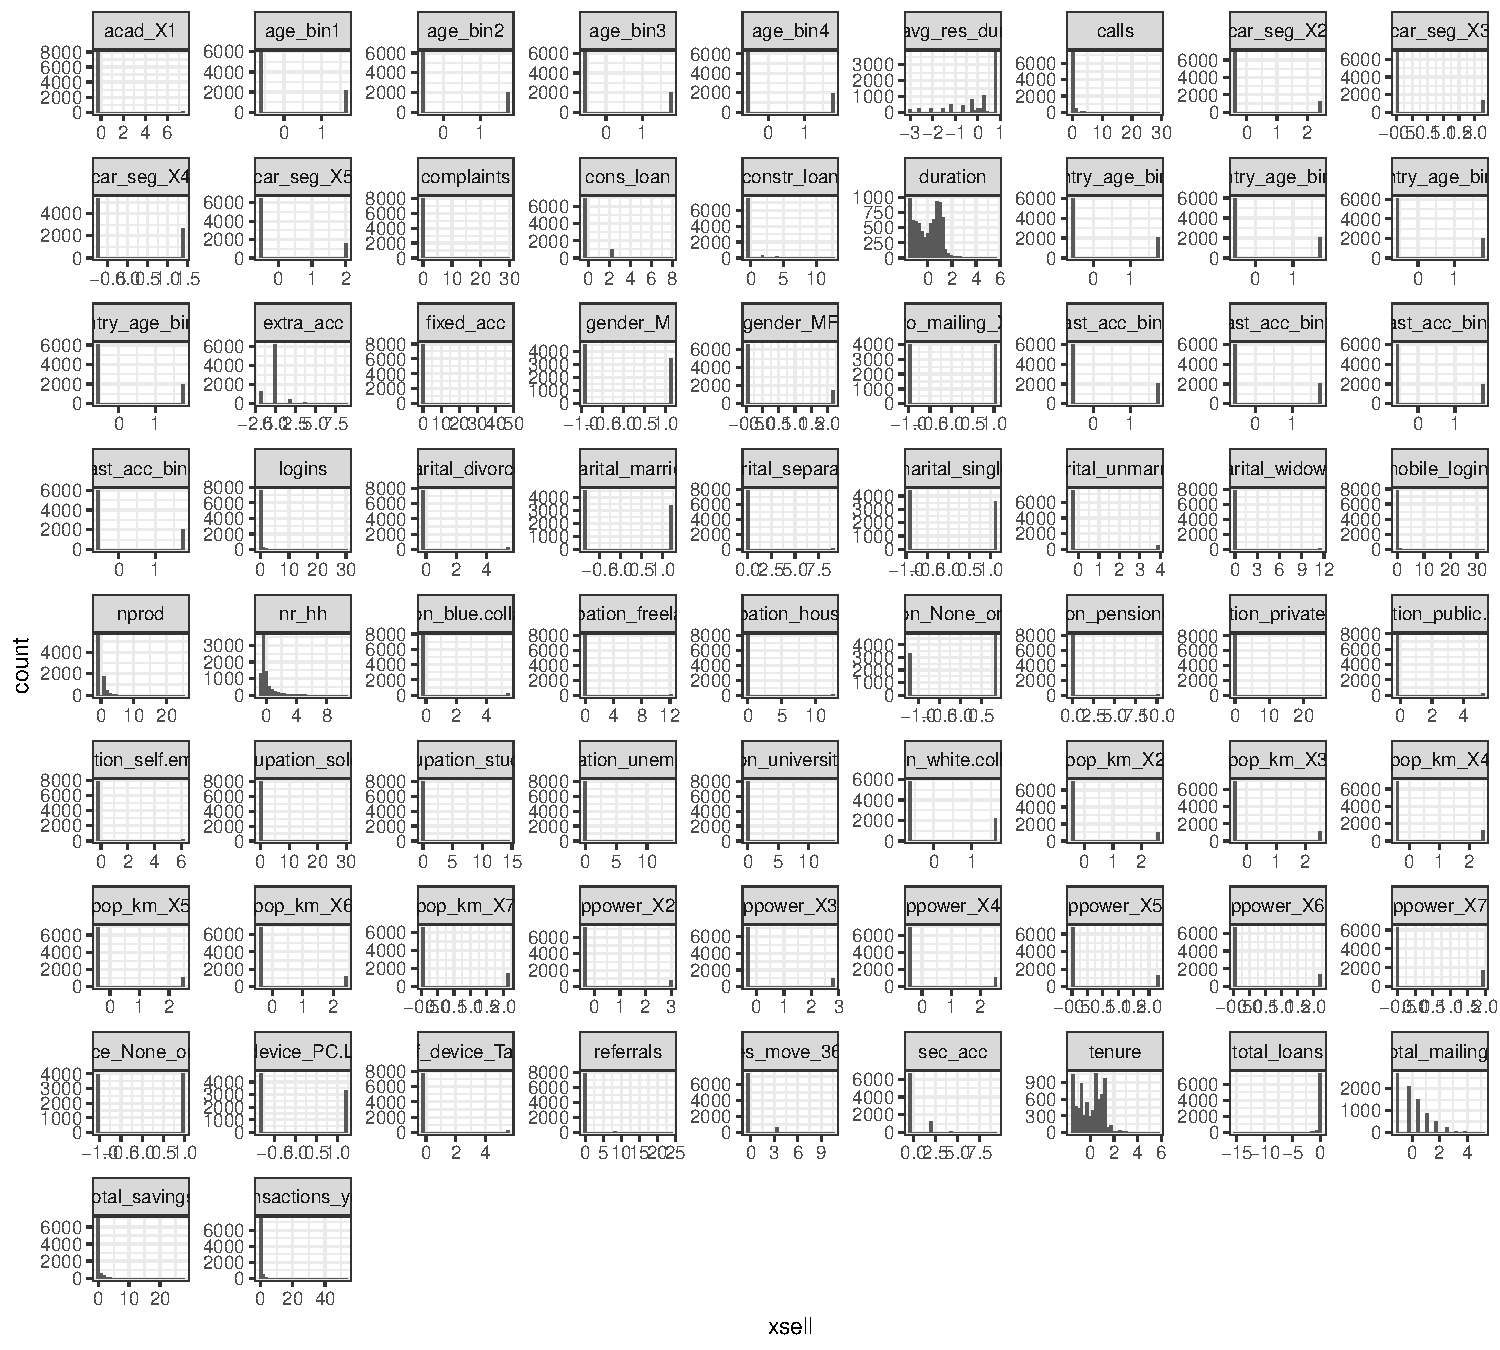
\includegraphics[scale=0.63]{figures/hist_all_features.pdf}
	\caption{Histogram of all features after feature engineering process}
	\label{fig_hist}
\end{figure}Figure \ref{fig_hist} displays the histograms for each
of those features.

\subsection{Artificial Neural Network with Keras}

While the previous section discussed the steps required to transform the data to a suitable format for an ANN,
this section will describe the basic architecture of this classification method.
This study uses the \proglang{R} interface \pkg{keras} \citep{cholletInterfaceKeras2017} to the popular same name \proglang{Python} library.
This high-level API enables an easier way to access the features of Google's \pkg{TensorFlow} \citep{abadiTensorFlowLargeScaleMachine2015}.

The neural network in this study is a common feedforward network which uses the backpropagation algorithm to adjust its weights \citep{werbosBackpropagationTimeWhat1990}.
Based on the feature engineering process described in the previous chapter, the ANN has $n_x = 74$ inputs $X_i$, 
two hidden layers with neurons $H_i^l$ referring to the $i^{th}$ neuron in the $l^{th}$ hidden layer. 
The number of neurons in the hidden layers is subject to hyperparameter tuning in the following section.
As a final layer, the ANN predicts the single output $\hat{Y}_i$, in our case \code{xsell}.
Figure \ref{fig_nn_arch} graphically visualizes the architecture.
\begin{figure}
\begin{center}
\def\layersep{3.5cm}

\begin{tikzpicture}[
   shorten >=1pt,->,
   draw=black!50,
    node distance=\layersep,
    every pin edge/.style={<-,shorten <=1pt},
    neuron/.style={circle,fill=black!25,minimum size=17pt,inner sep=0pt},
    input neuron/.style={neuron, fill=green!50},
    output neuron/.style={neuron, fill=red!50},
    hidden neuron/.style={neuron, fill=blue!50},
    annot/.style={text width=4em, text centered}
]

    % Draw the input layer nodes
    \foreach \name  [count=\y] in 
    {acad\_X1, age\_bin1, \dots,  age\_bin4, mobile\_logins, tenure, \dots, total\_mailings, transactions\_year}
     {   \node[input neuron, pin=left:\name] (I-\y) at (0,-\y cm) {};  
     }

    % set number of hidden layers
    \newcommand\Nhidden{2}
    \newcommand\NodOne{5}
    \newcommand\NodTwo{10}
    \newcommand\Nod{9}

    % Draw the hidden layer nodes
%    \foreach \N in {1,...,\Nhidden} {

     \foreach \y in {1,...,\NodOne} {
          \path[yshift=-1.80cm]
              node[hidden neuron] (H1-\y) at (1*\layersep,-\y cm) {};
              }
    \node[annot,above of=H1-1, node distance=2.8cm] (hl1) {Hidden layer 1};
     \foreach \y in {1,...,\NodTwo} {
          \path[yshift=0cm]
              node[hidden neuron] (H2-\y) at (2*\layersep,-\y cm) {};            
           }
    \node[annot,above of=H2-1, node distance=1cm] (hl2) {Hidden layer 2};          

%    }

    \node[below=3.2cm of H1-\NodOne] (text1) {64 neurons};
    \node at (text1 -| H2-1) (text2) {128 neurons};
	\node at (text1 -| I-9) (text1) {74 inputs};

    % Draw the output layer node
    \node[output neuron,pin={[pin edge={->}]right:xsell}, right of=H\Nhidden-5] (O) {};

    \node at (text1 -| O) (text3) {1 output};
    % Connect every node in the input layer with every node in the
    % hidden layer.
    \foreach \source in {1,...,9}{
        \foreach \dest in {1,...,\NodOne}{
            \path (I-\source) edge (H1-\dest);
         }
    }
    % connect all hidden stuff
    \foreach [remember=\N as \lastN (initially 1)] \N in {2,...,\Nhidden}
       \foreach \source in {1,...,\NodOne}
           \foreach \dest in {1,...,\NodTwo}
               \path (H\lastN-\source) edge (H\N-\dest);

    % Connect every node in the hidden layer with the output layer
    \foreach \source in {1,...,\NodTwo}
        \path (H\Nhidden-\source) edge (O);

    % Annotate the layers

    \node[annot,left of=hl1] {Input layer};
    \node[annot,right of=hl\Nhidden] {Output layer};
\end{tikzpicture}
% End of code
\label{fig_nn_arch}
\caption{Architecture of the Artificial Neural Network implemented in this study}
\end{center}
\end{figure} \label{fig_nn_arch}
This network uses a random uniform distribution $U(-0.05, 0.05)$ to initialize the weights for each neuron $H_i^l$.
Also, a bias initialized at zero feeds into the two hidden layers, for which each $H_i^l$ is activated by a rectifier function (\code{ReLU}).
\cite{glorotDeepSparseRectifier2011} show that rectifying units in an ANN yield superior outcomes compared to others such as the hyperbolic tangent activation function. Since the output $\hat{Y}_i$ is a binary feature in this case, I use a sigmoid activation function for the output layer.
To avoid overfitting, the model implements dropout for the hidden layers.
This process randomly drops units from the ANN and thus leads to a more generalizable model \citep{srivastavaDropoutSimpleWay2014}.
Mitigating the risk of overfitting to the training data is also one key objective of the next section.

\subsection{Cross-validation and Hyperparameter Tuning} \label{sec_crossval}
After setting up the basic architecture of the neural net, this section describes the process that leads to the \textit{best} model\footnote{as mentioned earlier, this is not the best model \textit{existing}, but \textit{found}.}.
An important feature of the \textit{best} model is that it does not memorize the exact relationships in the training data set---overfitting---but
rather learns the generalizable underlying mechanisms an thereby performs well on the holdout validation data set. 
For this purpose I first describe the optimization of the ANN through cross-validating predictions of several training epochs on a holdout 
sample and then introduce hyperparameter tuning---a process that leads to the most desirable configuration of the ANN by
running many combinations of model specifications.

To compile the ANN, I use the adaptive moment estimation algorithm \code{Adam} \citep{kingmaAdamMethodStochastic2014}
which is recommended as the go-to gradient descent optimizer \citep{ruderOverviewGradientDescent2016}.
This optimizer minimizes the cross-entropy loss \citep{zhangGeneralizedCrossEntropy2018} for each training epoch and accordingly updates the weights
for the next model.
Figure \ref{fig_history} shows the training history of the chosen ANN over ten epochs and the cross-entropy loss in the top pane, and the accuracy
in the bottom part, each for the training and validation data set.

\begin{figure}[ht]
	\centering
  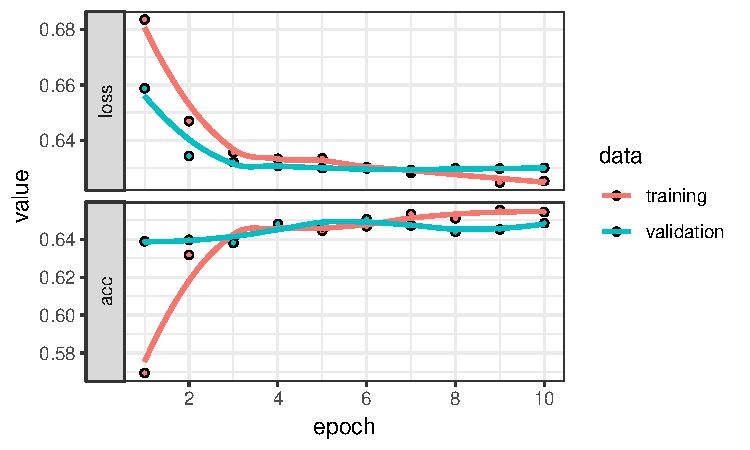
\includegraphics[scale=0.8]{figures/train_history.pdf}
	\caption{Loss and accuracy for training and test data over training history of the tuned model}
	\label{fig_history}
\end{figure}
The validation accuracy in comparison with the training accuracy in this case indicates first how accurate the ANN predicts true positives 
and true negatives in both data sets, but more importantly, gives an indication whether overfitting is an issue.
If the training accuracy kept steadily increasing, while the validation accuracy kept relatively constant, the model would overfit---which means
that the model is not generalizable beyond the training data set \citep{hansenNeuralNetworkEnsembles1990}.
As exhibited in figure \ref{fig_history}, both accuracies are relatively constant and equal during the last training epochs.
This is a strong indication that the model does not overfit and will perform similarly on the test or out-of-time data.

However, one question remains unanswered with cross-validation: Which model architecture leads to the most accurate predictions?
Hyperparameter tuning provides a remedy to this issue \citep{bergstraRandomSearchHyperparameter2012}.
In short, this process runs numerous models with combinations of hyperparameters\footnote{Hyperparameters refer to the specifications of an ANN,
such as number of units per hidden layer, dropout rate and weights, but also different optimization algorithms and activation functions \citep{bengioGradientbasedOptimizationHyperparameters2000}}. 
The model with the highest \code{val\_acc} is then chosen to be the \textit{best} model for prediction of \code{xsell}.
This study uses the "naive" grid method, which runs all possible combinations of pre-defined values for hyperparameters\footnote{I use each three different values of the hyperparameters \code{val\_acc}, \code{acc}, \code{units1}, \code{dropout1}, \code{units2}, \code{dropout2}, \code{epochs} and \code{batch}}.
However, this method is computationally expensive.
It requires $N=a^b$ different models, where $a$ is the number of discrete values for each parameter and $b$ is the 
number of hyperparameters to be tuned.
Running two separate sets of hyperparameter combinations for 324 different models took roughly five hours on a standard consumer laptop.
It can be assumed that this limited set of combinations did by far not yield the best model.
However, this naive grid method needs an exponentially increasing number of different models and thus gets difficult to handle quite quickly.
A possible solution to this problem is random search, which is even more efficient than grid search \citep{bergstraRandomSearchHyperparameter2012}.

By cross-validating the predictions with a loss function and by tuning the ANN's hyperparameter, 
this section described the approach to finding the most suitable model for the prediction task at hand.
The next part turns to prediction explanation---a key discussion point and critique of neural networks

\subsection{Local Interpretable Model-agnostic Explanation (LIME)}
In contrast to traditional regression-based methods that yield beta-coefficients and enable the construction of a functional form of 
the underlying mechanisms in the data, a neural network does not provide an easily interpretable function that links $Y_i$ to $X_i$.
A common criticism of ANN hence is the "black-box"-argument \citep{benitezAreArtificialNeural1997, dayhoffArtificialNeuralNetworks2001}.
Though the model might yield more accurate predictions, there is no clear answer to the question why the model predicted those particular values
or which features contributed by how much to that.

With the development of new methods that address this problem, an ANN is less a black box.
Consistent with the research question to uncover factors that drive cross-sell, 
this section focuses on the Local Interpretable Model-agnostic Explanation (LIME) introduced by \cite{ribeiroWhyShouldTrust2016a} as a methodology
to assess factor importance on a single customer level\footnote{Other tools such as neural interpretation diagrams, Garson's algorithm, sensitivity analysis or randomized approaches
\citep{oldenIlluminatingBlackBox2002} offer similar explanations on an aggregate level. However, covering those is beyond the scope of this paper.}.
LIME uses a trick to come up with an interpretable explanation: While the highly non-linear function of the ANN is unknown over the total space,
it can be approximated locally by an easier, readily interpretable model such as a linear regression or a decision tree.

While those models do match the functional form of the neural network at all globally, they can yield accurate \textit{local} approximations
\citep[see figure 3 for a visual example]{ribeiroWhyShouldTrust2016a}.
Turning to the task at hand, this paper uses a multiple linear regression with the ten most important features for every customer.
LIME permutes every observation and calculates the \code{gower}-distance between the observation and the permutation \citep{pedersenUnderstandingLime2018}.
It then fits a forward-selection procedure on the basis of a ridge regression \citep{pedersenPackageLimeLocal2018} to identify the ten most 
important features, weighted by the distance calculated earlier.
Following \cite{ribeiroWhyShouldTrust2016a}, the linear regression coefficients are then reported as a locally accurate approximation of feature importance.
This method hence enables to go beyond the typical "black-box" description of a neural network.
While this chapter described the implemented methods theoretically, the remainder of this paper reports and interprets the results of those 
machine learning techniques applied on the cross-sell data set.

\section{Results and Model Comparison}
This section proceeds as follows: First, it reports the results of the hyperparameter tuning and cross-validation and the resulting optimal ANN architecture.
The second part then compares the predictions of the described neural network to a simple benchmark logit model.
It concludes by reporting the feature importance for individual customers derived by LIME.

\subsection{Choosing the Neural Network Architecture}
The task of choosing the \textit{best} ANN architecture is not trivial. 
Using the approach described in section \ref{sec_crossval}, I ran a total of 324 different models, each with different combinations of hyperparameters.
Ranked by $val\_acc$, table \ref{tab_hypertune} shows the top five and bottom two models by validation accuracy with respective model specifications.
\begin{table}[!htbp] \centering 
  \caption{Resulting statistics of 324 hyperparameter tuning model runs} 
  \label{tab_hypertune} 
\begin{tabular}{@{\extracolsep{5pt}} ccccccccc} 
\\[-1.8ex]\hline 
\hline \\[-1.8ex] 
rank & val\_acc & acc & units1 & dropout1 & units2 & dropout2 & epochs &batch \\ 
\hline \\[-1.8ex] 
1 & $0.656$ & $0.654$ & $64$ & $0.600$ & $128$ & $0.600$ & $10$ & $100$ \\ 
2 & $0.654$ & $0.692$ & $128$ & $0.600$ & $64$ & $0.600$ & $30$ & $150$ \\ 
3 & $0.653$ & $0.674$ & $64$ & $0.600$ & $64$ & $0.600$ & $30$ & $100$ \\ 
4 & $0.651$ & $0.658$ & $64$ & $0.600$ & $64$ & $0.600$ & $10$ & $100$ \\ 
5 & $0.651$ & $0.673$ & $64$ & $0.600$ & $128$ & $0.600$ & $30$ & $50$ \\ 
$\dots$ & $\dots$ & $\dots$ & $\dots$ & $\dots$ & $\dots$ & $\dots$ & $\dots$ & \dots  \\
323 & $0.604$ & $0.731$ & $64$ & $0.200$ & $32$ & $0.400$ & $30$ & $128$ \\ 
324 & $0.602$ & $0.735$ & $64$ & $0.200$ & $32$ & $0.200$ & $30$ & $128$ \\ 
\hline \\[-1.8ex] 
\end{tabular} 
\end{table} 
It is noteworthy that this evaluation metric only varies by five percentage points from the best ($65.6\%$) to the worst model ($60.2\%$).
Also, the dropout rate for all best performing models is $0.6$ for both hidden layers, while the number of units in those varies between $64$ and $128$ 
for both layers between input and output.
In contrast to that the least preferable models exhibit only $32$ neurons in the second hidden layer.
In this case, a higher number of neurons in those layers appears to better capture the effects of the input features on \code{xsell}.
The winning model used ten training epochs, that means the model ran ten times before stopping.
This value is rather low\footnote{I tried epoch values of 5, 10, and 30 for the tuning routine.} and suggests an advantage of stopping early to avoid overfitting. 
Finally, the size of the batches---that is the number of samples sent back and forth through the network at once\citep{cholletInterfaceKeras2017}---apppears to not have an obvious impact
on model performance. 


Even though this routine identified the best out of 324 models, it only tested three different values for eight hyperparameters in two seperate runs.
Due to the computational complexity, important parameters such as the $learning rate$ was not included.
Furthermore, I only tested three more or less arbitrarily chosen discrete values for the included model characteristics---it is therefore obvious that
better models do exist. It is however difficult to identify them with the grid method and limited computational resources.

\subsection{Comparing the Predicions of the ANN with the Benchmark Logit Model}

The ANN from the previous section with the highest validation accuracy is furthermore applied to the remaining unseen test data\footnote{20\% 
of the 10,000 observations in the data set were used for testing, while the remaining 8,000 observations form the training set. Out of those, I reserved
2,400 rows (30\%) as a holdout validation sample for cross-validation during the fitting process}.
To assess the quality of the model, this paper now compares the resulting model statistics and confusion matrices of the discussed ANN with those of a 
simple logit model based on the same 74 input features in the neural network\footnote{In fact, this logit model has a relatively simple functional form, 
since it throws in every feature at hand without any selection mechanism or concern for multicolllinearity.
However, those features have undergone the same extensive feature engineering process as described for the ANN.
Hence, a lot of concerns are dealt with, e.g. though not functionally mapped, the logit model incorporates non-linear effects of \code{age} through binning.}.
Table \ref{tab_comparemodel} displays all relevant model performance metrics from accuracy to kappa and each confusion matrix.
To a surprise, there is no apparent difference in model accuracy between the hyperparameter tuned ANN and the simple benchmark logit model.
The reference model even predicts \code{xsell} 0.4 percentage points more accurate\footnote{Due to the small test set sample size of 2,000 this 
effect might not be statistically significant.}.
Since 50\% of all customers in the data set made a purchase, this is the benchmark accuracy for any predictive model.
Both the ANN and logit model in this case yield a roughly 29\% increase in accuracy compared to a coin toss.
%Comparison of Model Statistics
\begin{table}[!htbp] \centering
\caption{Model performance comparison---statistics and confusion matrix}
\label{tab_comparemodel} 
{\small
\begin{tabular}{@{\extracolsep{5pt}} ccccccccc} 
\\[-1.8ex]\hline 
\hline \\[-1.8ex] 
\multicolumn{3}{c}{\textit{Benchmark Logit}} & \multicolumn{3}{c}{\textit{Hyperparameter-tuned ANN}} \\ \hline
Accuracy & 0.6463 &  & Accuracy & 0.6423 &  \\
Sensitivity & 0.6653 &  & Sensitivity & 0.7331 &  \\
Specificity & 0.6271 &  & Specificity & 0.5508 &  \\
Pos Pred Value & 0.6429 &  & Pos Pred Value & 0.6221 &  \\
Neg Pred Value & 0.6500 &  & Neg Pred Value & 0.6716 &  \\
Kappa & 0.2925 &  & Kappa & 0.2841 &  \\
Prevalence & 0.5023 &  & Prevalence & 0.5023 &  \\
\hline \\[-1.8ex] 
 & \multicolumn{2}{c}{\textit{Actual}} &  & \multicolumn{2}{c}{\textit{Actual}} \\
\multicolumn{1}{r}{\textit{Prediction}} & 0 & \multicolumn{1}{c}{1} & \multicolumn{1}{r}{\textit{Prediction}} & 0 & \multicolumn{1}{c}{1} \\ 
\multicolumn{1}{r}{0} & 624 & \multicolumn{1}{c}{336} & \multicolumn{1}{r}{0} & 548 & \multicolumn{1}{c}{268} \\
\multicolumn{1}{r}{1} & 371 & \multicolumn{1}{c}{668} & \multicolumn{1}{r}{1} & 447 & \multicolumn{1}{c}{736} \\
\hline \\[-1.8ex] 
\end{tabular}
}
\end{table}
Nevertheless, both models produce structurally different predictions.
This becomes clear when comparing sensitivity (true positive rate) and specificity (true negative rate).
The ANN is relatively better at predicting customers that actually buy another product (\code{xsell = 1}),
while the logit model more accurately predicts negative outcomes.
This has far-reaching implications for business applications, which are further elaborated on in chapter~\ref{sec_man_impl}.

Another widely used visual tool and metric for model comparison in machine learning is the receiver operating characteristics curve (ROC) and the associated
area under curve (AUC) \citep{fawcettIntroductionROCAnalysis2006}.
Figure \ref{fig_roc} plots both ROC curves and the AUC in a single plot---the curves are visually inspected almost identical.
Quantified by the AUC, the ANN performs 0.9 percentage points better than the logit model at 69.3\%.

\begin{figure}[ht]
	\centering
  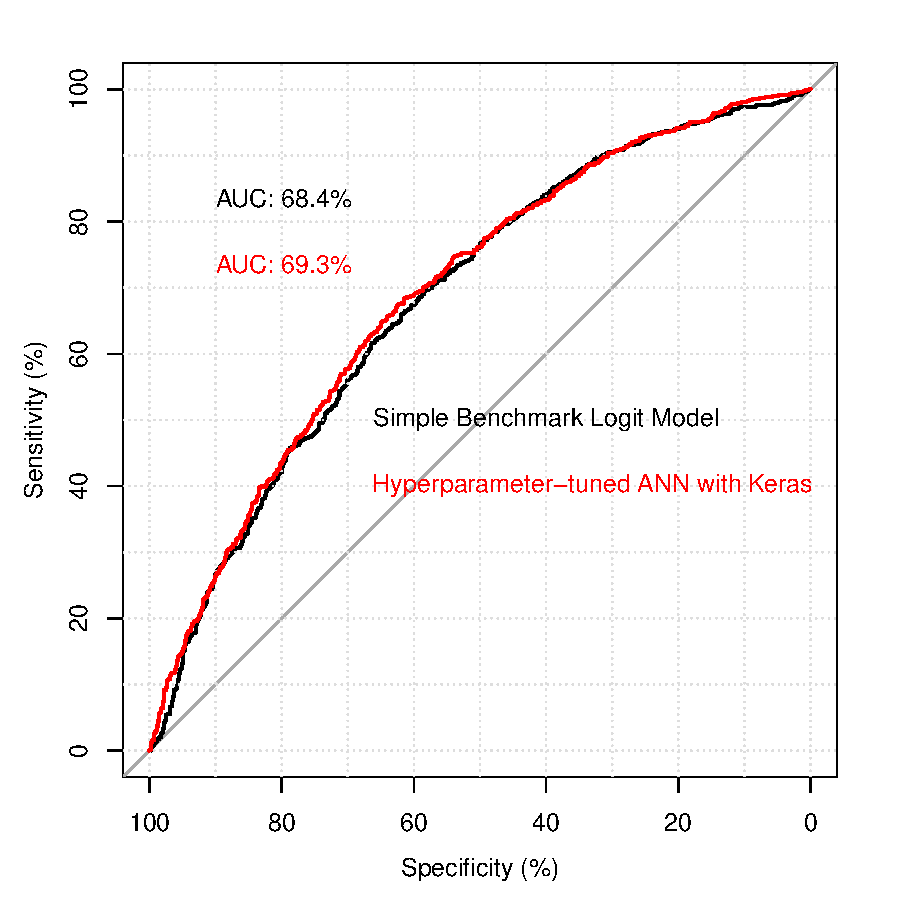
\includegraphics[scale=0.63]{figures/roc_auc_comp.pdf}
	\caption{ROC curve comparison between benchmark logit and hyperparameter-tuned neural network predictions}
	\label{fig_roc}
\end{figure}





\subsection{Beyond the Black Box: Feature Importance with LIME}

\begin{figure}[ht]
	\centering
  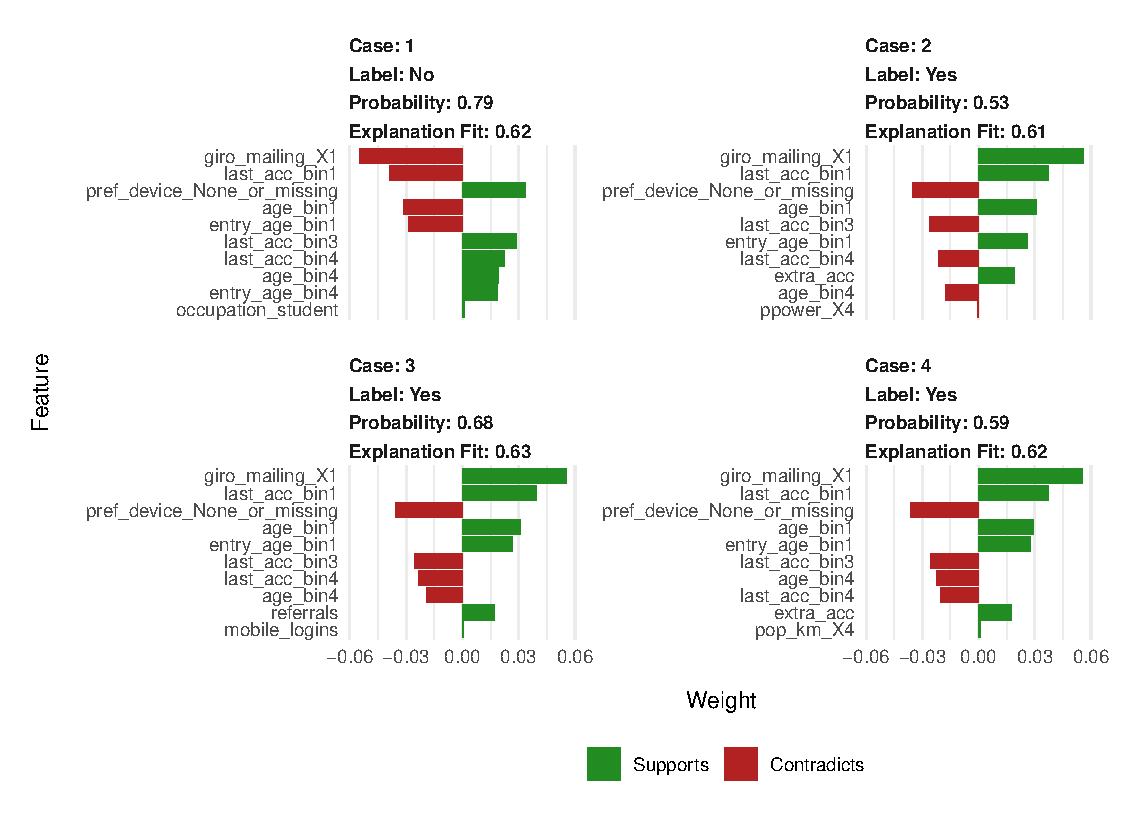
\includegraphics[scale=0.83]{figures/lime_first_four.pdf}
	\caption{LIME feature importance of the ten most important features for each of the first four customers in the test data set}
	\label{fig_lime_four}
\end{figure}

\begin{figure}[ht]
	\centering
  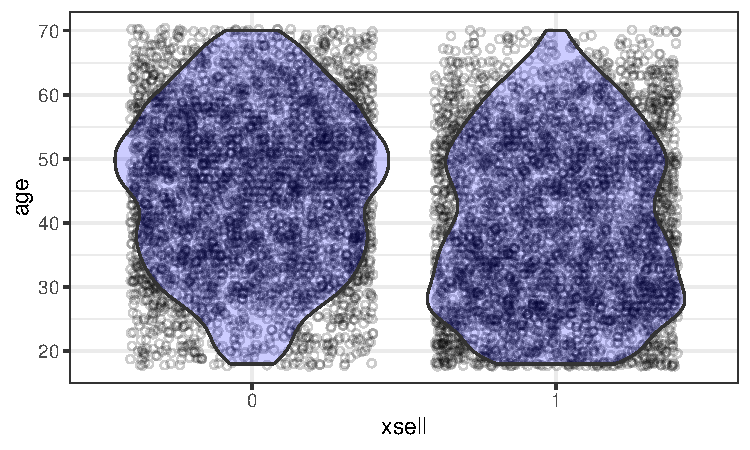
\includegraphics[scale=0.83]{figures/violin_age_xsell.pdf}
	\caption{Individual variable assessment---violin plot of xsell vs. age}
	\label{fig_lime_four}
\end{figure}




\section{Managerial and Research Implications} \label{sec_man_impl}
Include discussion of sensitivity vs. specificity here.
\section{Conclusion}




\clearpage
\appendix
\section{Appendix}
\begin{figure}[ht]
	\centering
  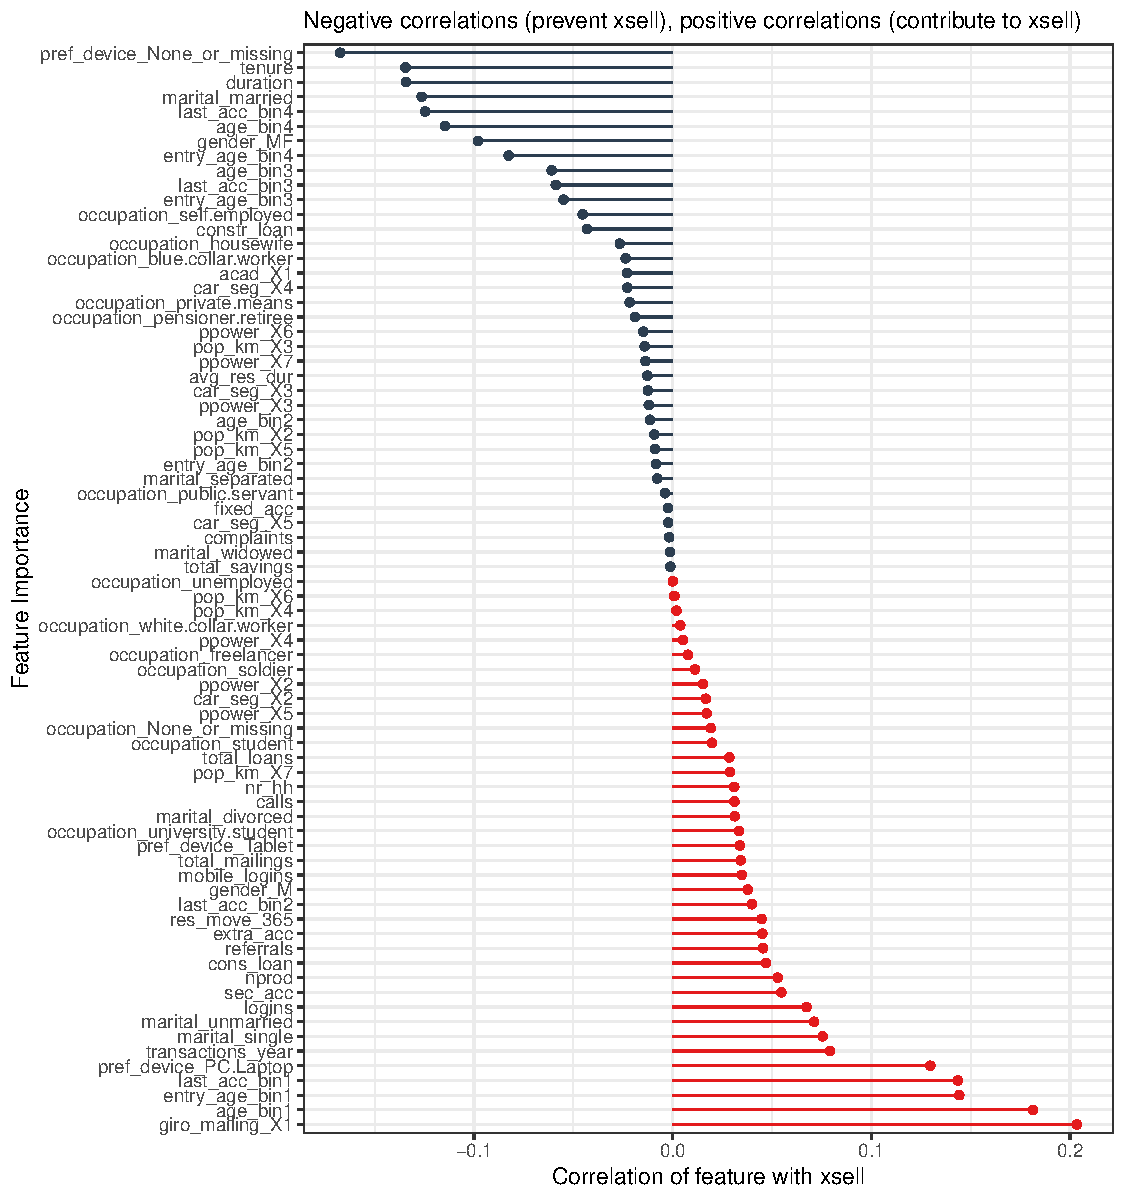
\includegraphics[scale=0.8]{figures/corrplot.pdf}
	\caption{Correlation of feature engineered variables with xsell}
	\label{fig_corr}
\end{figure}


\clearpage
\bibliography{library}

\newpage
\thispagestyle{empty}
\section*{Statutory Declaration}\label{statutory-declaration}

I herewith declare that I have completed the present thesis independently, without making use of
other than the specified literature and aids. Sentences or parts of sentences quoted literally are
marked as quotations; identification of other references with regard to the statement and scope of
the work is quoted. The thesis in this form or in any other form has not been submitted to an examination body and has not been published.
This thesis has not been used, either in whole or part, for another examination achievement.

\vspace{1cm}

Frankfurt am Main, July 31, 2019
\vspace{2cm}

. . . . . . . . . . . . . . . . . . . . . . . . . . . . . . .
\vspace{0.1cm}

Lukas J\"urgensmeier
\end{document}
